\section{HTML Templates}\label{html-templates}

\todo{Buchquelle hinzufügen [S.101-107]}

Bisher gibt es ohne eine Library oder Framework keine Möglichkeit, im Browser Templates zu rendern, um bestimmte Inhalte der Seite zur Laufzeit auszuwechseln. Die Technologie ``\ac{HTML} Templates'' ist eine neue Technologie im Rahmen der Web Components und versucht eben dieses Problem mit einer nativen \ac{API} zu lösen.

Im Kontext der Entwicklung einer \ac{MVC}-Applikation ist der Mechanismus der Darstellung der Präsentations-Schicht, auch View genannt, besonders wichtig. Bisher ist dies ohne weiteres problemlos serverseitig in PHP, Ruby oder ähnlichem möglich, da diese Sprachen für die Webentwicklung eine Syntax für die Einbettung dynamischer Inhalte in \ac{HTML} bieten, die sogenannten Templates. Im Gegensatz zu den serverseitigen Technologien, existieren Client-seitige Lösungen bisher nur als Library oder Framework, wie beispielsweise Mustache.js oder Handlebars.js \cite{citeulike:13853015}. Eine native Möglichkeit, Templates auf der Client-Seite zu benutzen, fehlt bisher hingegen. An diese Problematik setzen die \ac{HTML} Templates an, durch welche diese Technik auch Einzug in den Browser erhält.

\begin{quote}
Das \ac{HTML} template-Element \textless{}template\textgreater{} dient dazu, Client-seitige Inhalte zu gruppieren, die nicht gerendert werden, wenn die Seite geladen wird, sondern anschließend zur Laufzeit mittels JavaScript gerendert werden können. Template kann als Inhaltsfragment aufgefasst werden, das für eine spätere Verwendung im Dokument gespeichert wird. \cite{citeulike:13852997}
\end{quote}


\subsection{Bisherige Umsetzung von Templates im Browser}\label{bisherige-umsetzung-von-templates-im-browser}

Dennoch gibt es diverse Methoden, diese Technologie im Browser zu simulieren. Diese sind jedoch eher als Hacks zu betrachten, da ihre eingesetzten Mittel nicht für dieses Problem gedacht sind. Sie bringen also einige Nachteile mit sich. Einige dieser Methoden werden nachfolgend aufgezeigt \cite{citeulike:13853018}.

\subsubsection{Via verstecktem \texttt{\textless{}div\textgreater{}}-Element}

Das Listing \ref{uetmedb} zeigt die Umsetzung eines Templates mit Hilfe eines \texttt{\textless{}div\textgreater{}}-Blocks, der via \ac{CSS} versteckt wird.

\lstinputlisting[language=HTML,label=uetmedb,caption=Umsetzung eines Templates mit einem \texttt{\textless{}div\textgreater{}}-Block]{kapitel2/listings/4-1.html}

Der entscheidende Nachteil dieser Methode ist, dass alle Ressourcen, also alle verlinkten Dateien, beim Laden der Webseite auch heruntergeladen werden. Zwar werden sie nicht angezeigt, dennoch verursachen sie eine große Datenmenge, welche initial übertragen werden muss. Dies geschieht in diesem Fall selbst wenn die Ressourcen eventuell erst später oder gar nicht benötigt werden, was eine massive Einschränkung der verfügbaren Bandbreite und Browser-Performance mit sich bringen kann. Des Weiteren kann es sich als schwierig erweisen, ein solches Code-Fragment zu stylen oder gar Themes auf mehrere solcher Fragmente anzuwenden. Eine Webseite, die das Template verwendet, muss alle \ac{CSS}-Regeln für das Template mit \texttt{\#mydivtemplate} erstellen, welche sich unter Umständen auf andere Teile der Webseite auswirken können. Eine Kapselung wird hier somit nicht vorgesehen.

\subsubsection{Via \texttt{\textless{}script\textgreater{}}-Element}

Eine weitere Möglichkeit ein Template umzusetzen besteht darin, den Inhalt eines Templates in ein \texttt{\textless{}script\textgreater{}}-Tag zu schreiben, wie in Listing \ref{uetmese} gezeigt.

\lstinputlisting[language=HTML,label=uetmese,caption=Umsetzung eines Templates mit einem \texttt{\textless{}script\textgreater{}}-Element]{kapitel2/listings/4-2.html}

Wie bei dem Beispiel mit einem \texttt{\textless{}div\textgreater{}}-Element wird auch bei dieser Methode der Inhalt nicht gerendert, da ein \texttt{\textless{}script\textgreater{}}-Tag standardmäßig die \ac{CSS}-Eigenschaft \texttt{display:\ none} hat. In diesem Fall werden jedoch die benötigten Ressourcen nicht geladen, somit gibt es keine zusätzlichen Performance-Einbrüche. Es besteht dennoch ein Nachteil, auf den besonders geachtet werden muss: Der Inhalt des \texttt{\textless{}script\textgreater{}}-Tags muss via \texttt{innerHTML} in den \ac{DOM} geklont werden, was eine mögliche \ac{XSS} Sicherheitslücke darstellen kann. Es muss also abgewägt werden, welche der Nachteile für den Entwickler am ehesten hinnehmbar sind und welche Methode verwendet werden soll.


\subsection{Das \texorpdfstring{\texttt{\textless{}template\textgreater{}}-Tag}{\textless{}template\textgreater{}-Tag}}\label{template-tag}

Den Problemen der oben genannten Methoden widmet sich der \texttt{\textless{}template\textgreater{}}-Tag, welcher eine native und sichere Methode für das Einbinden von dynamischen Inhalten etabliert. Das Template und die darin enthaltenen Inhalte werden beim Rendern des Webseite vollständig ignoriert, sie werden weder angezeigt, noch werden ihre benötigten Inhalte beim Laden der Webseite mitgeladen. Ebenso werden enthaltene JavaScripts nicht ausgeführt, auch kann JavaScript von außen nicht in das Template hinein traversieren. In Listing \ref{gsetmcssujs} wird die grobe Struktur eines einfachen Templates, das mit Hilfe des \texttt{\textless{}template\textgreater{}}-Tags umgesetzt wird, dargestellt.

\lstinputlisting[language=HTML,label=gsetmcssujs,caption=Grobe Struktur eines Templates mit \ac{CSS} und JavaScript]{kapitel2/listings/4-2.html}


\subsection{Benutzung}\label{benutzung}

Natürlich soll ein Template nicht nur im Quelltext stehen, damit es existiert, sondern es soll dynamisch zur Laufzeit geladen und gerendert werden. Dabei kann es an einer beliebigen Stelle im Quelltext stehen. Um es aus dem Quelltext in den \ac{DOM} zu importieren und zu rendern, muss es zunächst via JavaScript selektiert werden, was mit der Funktion \texttt{var\ template\ =\ document.querySelector('\#mytemplate');} möglich ist. Mit der Funktion \texttt{var\ templateClone\ =\ document.importNode(template.content,\ true);} wird eine Kopie als \ac{DOM}-Knoten des Templates erstellt. Als erster Parameter wird dabei der Inhalt des Templates (\texttt{template.content}) und als zweiter Parameter ein Boolean für \texttt{deep}, welcher angibt ob auch Kinderknoten geklont werden sollen. Nun kann der Inhalt des Templates mittels \texttt{document.body.appendChild(templateClone);} an einer beliebigen Stelle des \ac{DOM} eingefügt werden.


\subsection{Vorteile von HTML Templates}\label{vorteile}

Die Vorteile dieser nativen Implementierung für Templates sind vielfältig. So sind \ac{HTML} Templates ein fertiges Gerüst an \ac{HTML}, das nicht nachträglich mit JavaScript modifiziert werden muss, es kann aus dem Quelltext kopiert und beliebig oft und an beliebiger Stelle in den \ac{DOM} der Webseite eingefügt werden. Erst beim einfügen in den \ac{DOM} werden die Inhalte tatsächlich gerendert und Abhängigkeiten nachgeladen. Darunter fallen auch enthaltene Styles oder JavaScript-Codes, welche erst beim Einfügen angewendet und ausgeführt werden. So werden auch externe Stylesheets, JavaScript-Dateien oder Bilder und Videos erst dann geladen und abgespielt, wenn sie tatsächlich benötigt werden. Dadurch können auch beliebig viele \texttt{\textless{}template\textgreater{}}-Tags ohne signifikanten Performance-Einbruch im Quelltext stehen, da nur ihr Markup übertragen wird, es jedoch nicht vom Browser geparst werden muss. Des Weiteren sind Templates komplett vor dem \ac{DOM} versteckt, will man beispielsweise mit JavaScript in das Template mittels \texttt{document.getElementById('\#mytemplate\ .text')} hinein traversieren, so gibt die Funktion `null` zurück. Der abschließende und wohl auch größte Vorteil ist, dass mit JavaScript auf das Template zugegriffen werden und es an anderer Stelle dynamisch eingebunden werden kann.
Falls nun jedoch in einem Template mehrere weitere Templates geschachtelt sind, so muss jedes dieser Templates einzeln aus dem aktiven Template im \ac{DOM} kopiert und wieder eingefügt werden um es zu aktivieren.


\subsection{Browserunterstützung}\label{html-templates-browserunterstuetzung}

\ac{HTML} Templates sind zum Stand dieser Arbeit als einzige Technologie des Web Components Technology Stacks vom \ac{W3C} als Standard erklärt worden \cite{citeulike:13853159}. Somit ist auch die Browserunterstützung in den aktuellen Browsern, bis auf den Internet Explorer, sehr gut (siehe Abbildung \ref{fig:bdhtmltt}). Sie sind des Weiteren die einzige Technologie der Web Components, die bisher von Microsofts Edge ab Version 13 unterstützt werden.

\begin{figure}[htbp]
 \centering
 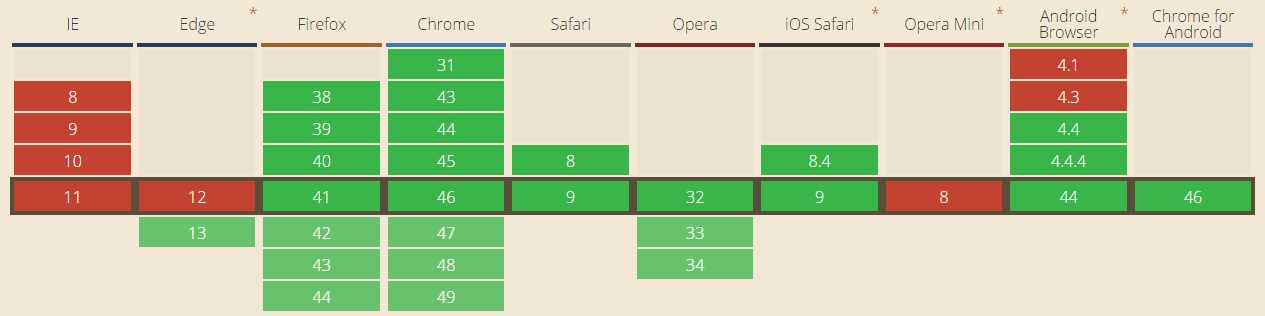
\includegraphics[width=\linewidth]{kapitel2/bilder/4-html-templates-browserunterstuetzung}
 \caption{Browserunterstützung des HTML Template Tags}
 \label{fig:bdhtmltt}
\end{figure}
